Как правило, стахастический градиентный спуск в чистом виде не используется. Обычно используют некоторые его модификации.

Одна из проблем классического градиентного спуска~--- биение вблизи точки экстремума. Проблема в том, что при приближении к точке минимума градиент не становится точне. Это можно исправить увеличением размера mini--batch'а при приближении к экстремуму, но очень сильно увеличить его размер мы не можем~--- вычислять очень дорого.

\subsection{Модификации стахастического градиентного спуска}

Пусть у нас есть некоторая очень сильно асцилирующая функция. По сути наш градинт и является такой функцией. Давайте попробуем сгладить имеющую функцию. Один из методов~--- экспоненциально взвешанная средняя.

\begin{center}
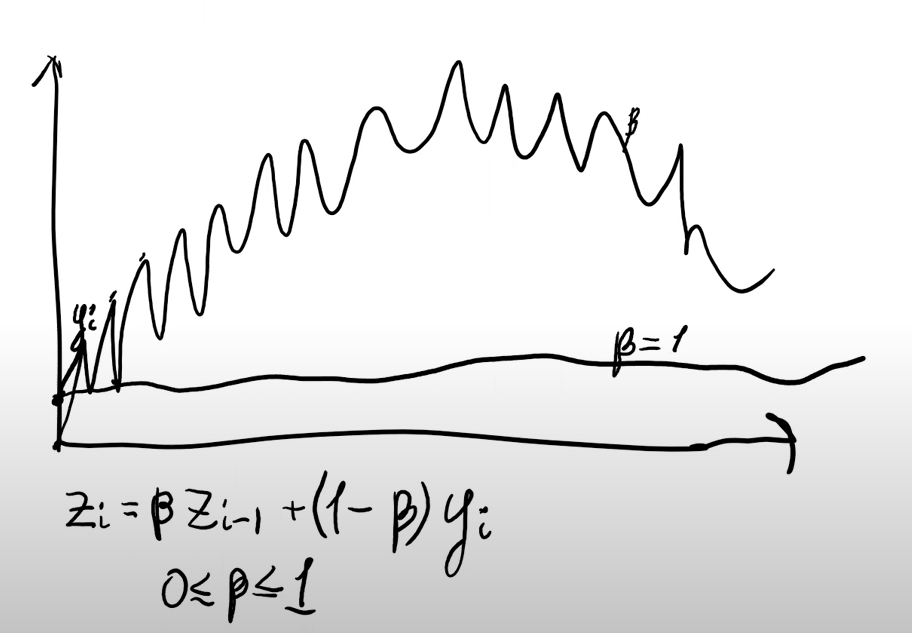
\includegraphics[scale=0.4]{img/exponential-median-method-function.png}
\end{center}

\subsubsection{SGD with momentum}

Пусть у нас есть некоторый вектор $g _i = \tl \nabla f (x_i)$, тогда $x_{i+1} = x_i - \alpha g_i$, где $\alpha$~--- learning rate.

$g_i = \beta g_{i - 1} + (1 - \beta) \tl \nabla f (x_i)$.

Другой вариант записи: $g_i = \beta g_{i - 1} + \alpha \tl \nabla f (x_i)$,~~~$x_{i+1} = x_i - g_i$.

Это имеет физическую аналогию. Пусть шарик катится вниз под действием иннерции

\subsubsection{Метод Нестерова}
Пусть у нас есть некоторая исходная точка. Из нее посмотрим туда, куда ведет нас энерция и из нее посмотрим туда, куда ведет нас градиент и сразу сделаем шаг на сумму векторов <<иннерции>> и градиента.

Для использования этого метода необходимо наложить много ограничений на функцию. Но иногда, функции подходят и тогда метод имеет квадратичную сходимость по сравнению с SGD with momentum.

\begin{center}
    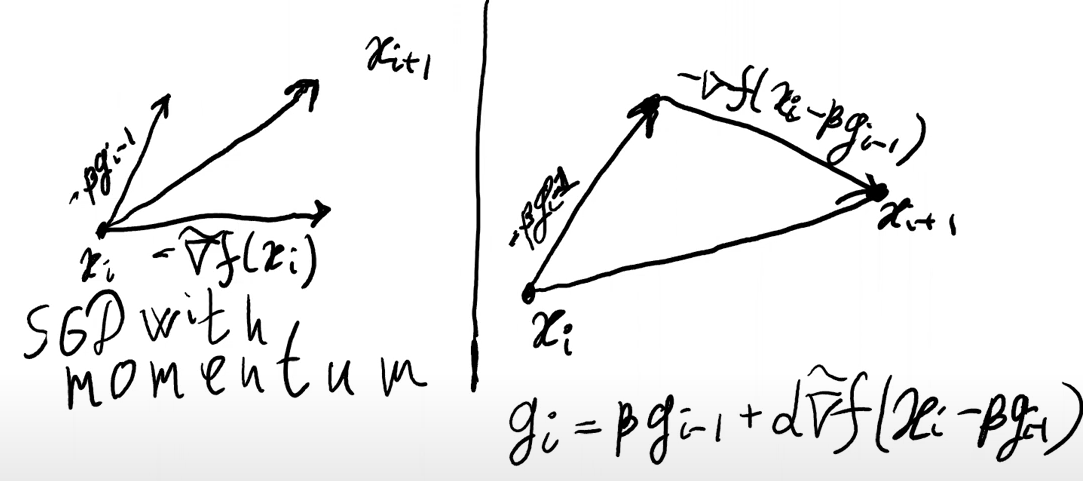
\includegraphics[scale=0.4]{img/sgd-with-moment-vs-nesterov.png}\\
    {Сравнение стахастического градиентного спуска с With moment и Nesterov модфикациями.}
\end{center}

\subsubsection{Ada Grad}
$v_i = v_{i - 1} + \left( \tl\nabla f (x+i) \right)^2$ (поэлементное возведение в квадрат).

$x_{i + 1} = x_i - \dfrac{\alpha}{\sqrt{v_i}}\tl \nabla (x_i)$ (корень тоже поэлементный).

Мы масштабируем разные элементы нашего градиента. Здесь мы сглаживаем не сам градиент, а в каком-то смысле его квадрат.

\subsubsection{RMS Prop (root min square propagation)}

Здесь мы усредняем квадрат градиента и при помощи этого сглаживаем функцию.

$v_i = \gamma v_{i - 1} + (1 -\gamma ) (\nabla f (x_i))^{2 (\mathrm{per~~element})}$.

$x_{i +1} = x_i - \dfrac{\alpha}{\sqrt{v_i}} \nabla f (x_i)$.

\subsubsection{Adam (Adavtive momvent estination, адаптивная оцнка моментов)}

$f_i = \beta_i g_{i - 1} + (1 - \beta_1) \tl \nabla f (x_i)$.

$v_i = \beta_2 v_{i-1} + (1 - \beta _2) \left(\tl\nabla f (x_i))\right)$.

$x_i = x_{i - 1} - \alpha \cdot \dfrac{g_i}{\sqrt{V_i} + \underbrace{\varepsilon}_{=10^{-8}}}$.

$\tl f_i = \dfrac{g_i}{1 - \beta_1 ^{i-1}}$,~~$ \tl v_i = \dfrac{v_i}{1 -\beta_{2}^{i-1}}$.

В качестве $\beta_1 = 0.9$, $\beta_2 = 0.999$.

\subsection{Резуляризация}

В чем Проблема? Хотим достаточно точно работать с функцией. Однако если взять функцию и получить у нее достаточно много точек, то окажется, что функция ведет себя крайне не красиво и не понятно, где искать у нее минимум. Эту задачу решает регуляризация.

\begin{center}
    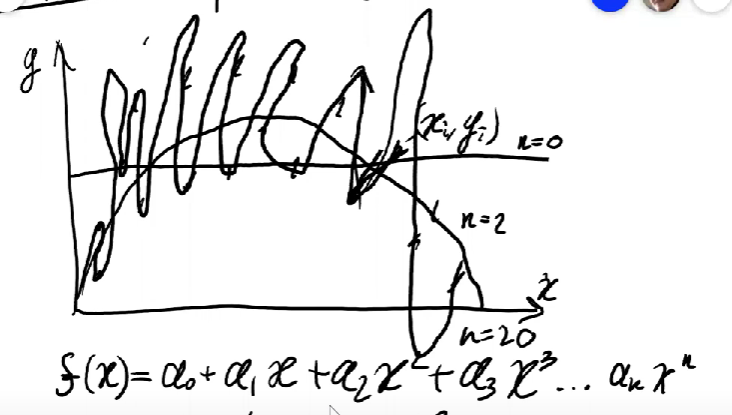
\includegraphics[scale=0.55]{img/regularisation-ex1.png}
\end{center}

Мы хотим представить в виде суммы полиномов.
Если возьмем большие степени, то будет много шума и переобучение, если очень маленькую, то будет неточно и недообучение. Хотим представить в виде такой суммы.

\[ L(\alpha) = \sum_i \left(f (x_i) - y_i \right)^2 \]

Один способ~--- представлять в виде суммы с штрафами за осциляцию.

\[ L (\alpha) = \sum_i \left( f (x_i) - y_i \right)^2 + \underbrace{\gamma \sum_{j=1}^n a_j^2}_{L_2 \text{ -- reg}, \| \alpha \|_2 }.  \]
